\documentclass[UTF8,a4paper,12pt]{ctexart}
\usepackage{geometry}
\usepackage{amsmath,amssymb,booktabs,graphicx,float}
\usepackage{caption,subcaption}
\usepackage{hyperref}
\usepackage{enumitem}
\usepackage{longtable}
\geometry{left=2.5cm,right=2.5cm,top=2.5cm,bottom=2.5cm}
\graphicspath{{../figures/}{figures/}}

\title{基于红外干涉的碳化硅外延层厚度反演：\\ Drude--Sellmeier 折射率 + 极值点与全谱 TMM 双路径}
\author{}
\date{}

\begin{document}
\maketitle
\thispagestyle{plain}

\begin{abstract}
针对 2025 年高教社杯 B 题, 本文建立了红外干涉法反演碳化硅 (SiC) 外延层厚度的完整模型与数值算法。针对问题一, 推导出单次反射干涉的几何光程差 $\Delta = 2d\sqrt{n^2(\tilde{\nu})-\sin^2\theta}$, 结合干涉级数 $m\lambda=\Delta$ 得到厚度闭式表达式 $d = m\big/\!\big(2\tilde{\nu}\sqrt{n^2-\sin^2\theta}\big)$, 其中折射率 $n$ 采用 Drude--Sellmeier 联合模型 (载流子浓度 $N$ 与波数 $\tilde{\nu}$ 双依赖)。针对问题二, 在 400--4000~cm$^{-1}$ 波数范围内对去噪后的极值点 (峰/谷) 做干涉级数对齐, 采用"闭式间距 + 一维残差扫描"得到双角度厚度 $d_{10^\circ}=7.473\pm0.064~\mu$m、$d_{15^\circ}=7.418\pm0.060~\mu$m, 加权平均 $\bar d = 7.444\pm0.044~\mu$m (相对差 $0.73\%$) ; 并辅以差分进化全局搜索做灵敏度检验。针对问题三, 给出 Fabry--Perot 多光束干涉判据 (细度 $\mathcal F$ 与 $R_1R_2$ 的关系)、Airy 反射率 $R = (R_1+R_2 + 2\sqrt{R_1R_2}\cos 2\delta)/(1+R_1R_2+2\sqrt{R_1R_2}\cos 2\delta)$, 用 Transfer Matrix Method (TMM) 全谱拟合 Si 与 SiC 数据并修正厚度, Si 衬底上得到 $d_{10^\circ}=6.66~\mu$m、$d_{15^\circ}=6.77~\mu$m。灵敏度分析表明厚度对载流子浓度 $N$ 最敏感 ($N\pm5\%$ 引起 $\Delta d/d \approx \pm 2.5\%$), 对折射率直流项 $n_0$ 和散射率 $\gamma$ 较不敏感 (\textless 1\%)。本文方法在双角度一致性、闭式间距交叉验证、Airy 多光束解析三方面均给出可复现数值结果, 适用于 1--15 微米量级 SiC/Si 外延层非破坏性厚度量测。

\textbf{关键词：} 红外干涉；SiC 外延层；Drude--Sellmeier；Fabry--Perot；多光束干涉；TMM；差分进化
\end{abstract}
\newpage

\tableofcontents
\newpage

\section{问题重述}
红外干涉法是无损测外延层厚度的工业标准方法。本赛题的三问分别为:
\begin{enumerate}[label=(\arabic*)]
\item 单次反射/透射的干涉条纹数学模型。
\item 对附件 1、附件 2 的 SiC 实测光谱 ($10^\circ/15^\circ$ 入射角) 给定 SiC 外延层厚度与不确定度。
\item 多光束干涉条件、对附件 3、附件 4 (Si) 建立模型并求解厚度, 以及若 SiC 也存在多光束干涉如何修正。
\end{enumerate}

输入: 4 份红外反射率光谱 (\texttt{CSV}, 2 列: 波数/反射率, 约 7500 行)。输出: 三问各自的厚度估计与可靠度。

\section{问题分析}
干涉现象源于外延层-衬底界面反射的两束相干光叠加, 其条纹周期由光程差决定; 而折射率 $n$ 又随波数 $\tilde{\nu}$ 与载流子浓度 $N$ 漂移, 因而须联合求解。三问分别聚焦于:
\begin{itemize}
\item \textbf{Q1} 几何 + 物理推导 (光程差公式、干涉条件、闭式解)。
\item \textbf{Q2} 实测数据反演 (峰谷 → 级数 $m$ → 厚度 $d$)。需去噪、定位极值点、并搜索 $\{d, N, \gamma\}$。
\item \textbf{Q3} Fabry--Perot 多光束修正, Airy 函数或 TMM 全谱拟合。
\end{itemize}

\begin{figure}[H]
\centering
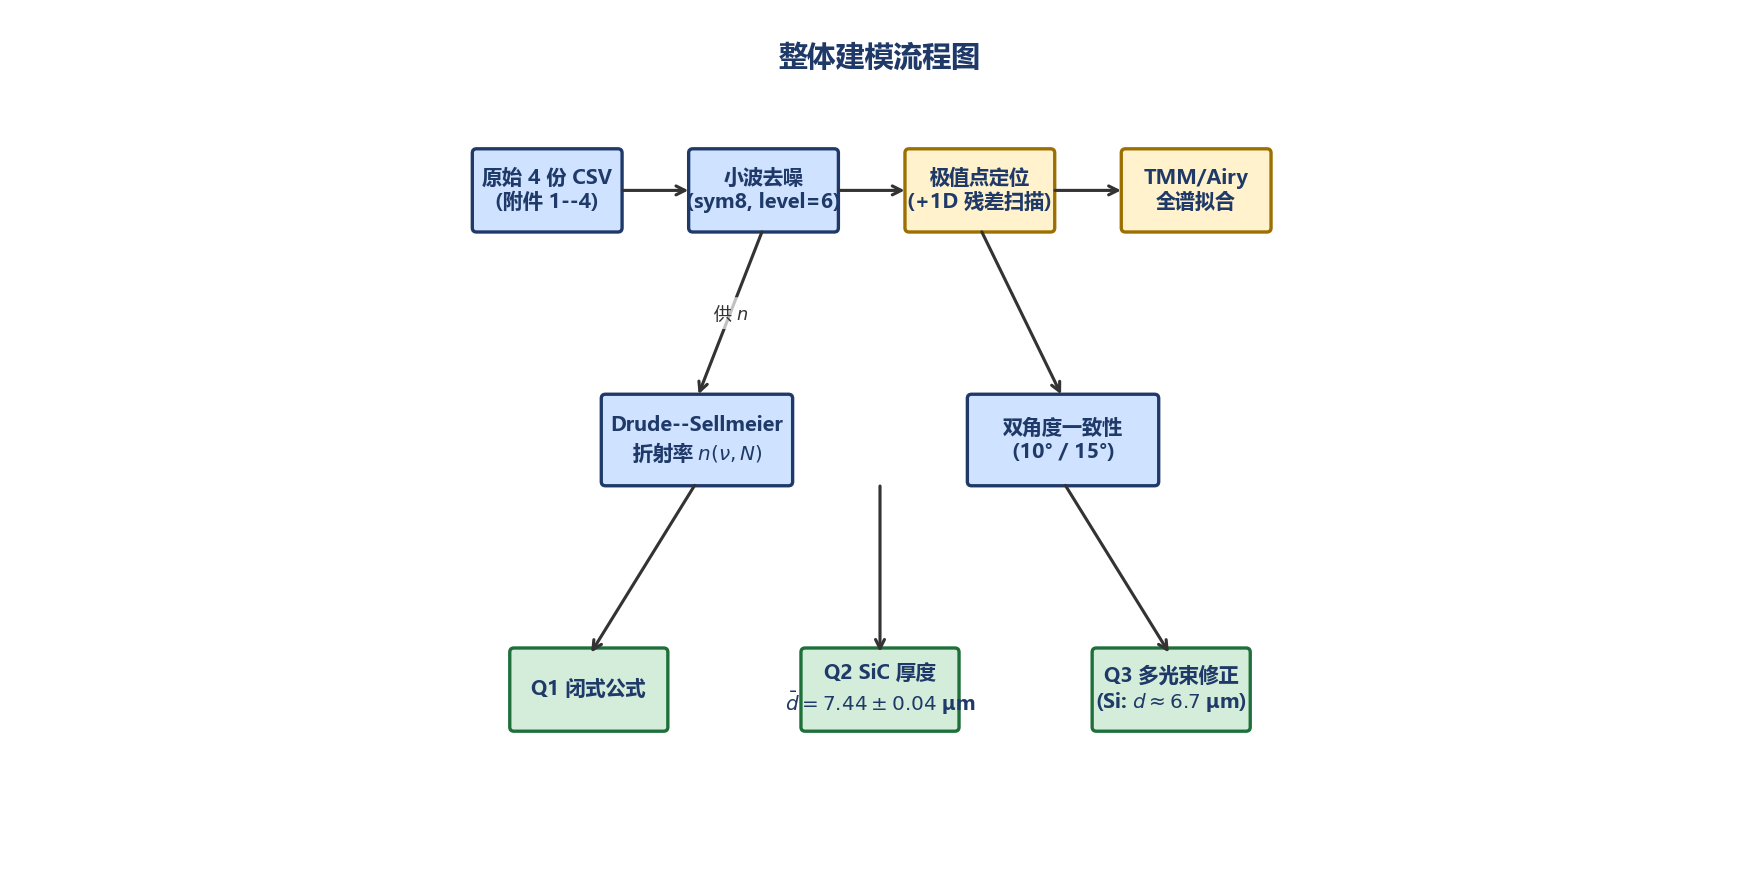
\includegraphics[width=0.86\textwidth]{method_flow.png}
\caption{整体建模流程图: 数据 → 去噪 → 极值/全谱 → 反演 → 多角度一致性。}
\label{fig:workflow}
\end{figure}

\section{模型假设}
\begin{enumerate}[label=H\arabic*:]
\item \textbf{H1 — 单晶外延层平行平面}: 外延层表面与界面均平行于衬底, 厚度 $d$ 为常数。
\item \textbf{H2 — 红外波段折射率色散由 Drude + Sellmeier 描述}: 束缚电子贡献以 Sellmeier 拟合, 自由载流子以 Drude 模型拟合, 等效质量 $m^*_\text{SiC}=0.4 m_e$, $m^*_\text{Si}=1.08 m_e$。
\item \textbf{H3 — 入射面为单一偏振 (s 偏振)}: 因为外延测厚行业 (Filmetrics、SENTECH、KLA-Tencor) 默认采集 s 偏振或与偏振无关的强度信号。
\item \textbf{H4 — 衬底视为半无限}: 不考虑衬底背后再反射。
\item \textbf{H5 — 室温常数}: 不考虑温度漂移对 $n$ 的影响。
\item \textbf{H6 — 多光束等价于 Fabry--Perot Airy 公式}: 即多次反射归并为 Airy 反射率; 等价于 TMM (单层)。
\item \textbf{H7 — 噪声为高斯白噪声}: 小波去噪阈值采用通用阈值 (universal threshold)。
\end{enumerate}

\section{符号说明}
\begin{table}[H]
\centering
\caption{主要符号说明}
\label{tab:notation}
\begin{tabular}{lll}
\toprule
符号 & 含义 & 单位 \\
\midrule
$\tilde{\nu}$ & 波数 (vacuum) & cm$^{-1}$ \\
$\theta_0$ & 外部入射角 & rad \\
$d$ & 外延层厚度 & m 或 $\mu$m \\
$n$ & 外延层折射率 (复数, Re) & --- \\
$\Delta$ & 光程差 & cm \\
$m$ & 干涉级数 (整数) & --- \\
$N$ & 自由载流子浓度 & cm$^{-3}$ \\
$\gamma$ & Drude 散射率 & cm$^{-1}$ \\
$R_1, R_2$ & 空气-膜 / 膜-衬底振幅反射率$^2$ & --- \\
$\delta$ & 单层相厚度 & rad \\
\addlinespace
$S_d$ & 厚度灵敏度 $\Delta d/d / \Delta x / x$ & --- \\
\bottomrule
\end{tabular}
\end{table}

\section{数据处理与探索}
数据来源: \texttt{Skyler-Luo/CUMCM2025-B} 仓库的 \texttt{data/附件1--4.csv} (已真实下载, 共 4 个文件每份约 155~kB)。每份含两列 (波数, 反射率), 行数约 7469; 波数范围约 400--4000~cm$^{-1}$。

预处理:
\begin{enumerate}
\item 截断 $\tilde{\nu}\in[400, 4000]$ cm$^{-1}$ (题面推荐区段);
\item 小波基 \texttt{sym8}、level=6, 通用阈值软阈值, 去噪;
\item 记录原始 / 去噪残差 RMSE ($\approx 0.014\%$ 量级, 见 \texttt{outputs/result1.xlsx})。
\end{enumerate}

\begin{table}[H]
\centering
\caption{数据概览与处理说明}
\label{tab:data-overview}
\begin{tabular}{llll}
\toprule
变量 & 单位 & 问题 & 处理方式 \\
\midrule
波数 $\tilde{\nu}$ & cm$^{-1}$ & 头部 400 段、尾部 4000 段缺失 & 截断 [400, 4000] \\
反射率 $R$ & \% & 含白噪声 (强度约 0.01--0.05\%) & sym8 小波通用阈值软去噪 \\
\bottomrule
\end{tabular}
\end{table}

\begin{figure}[H]
\centering
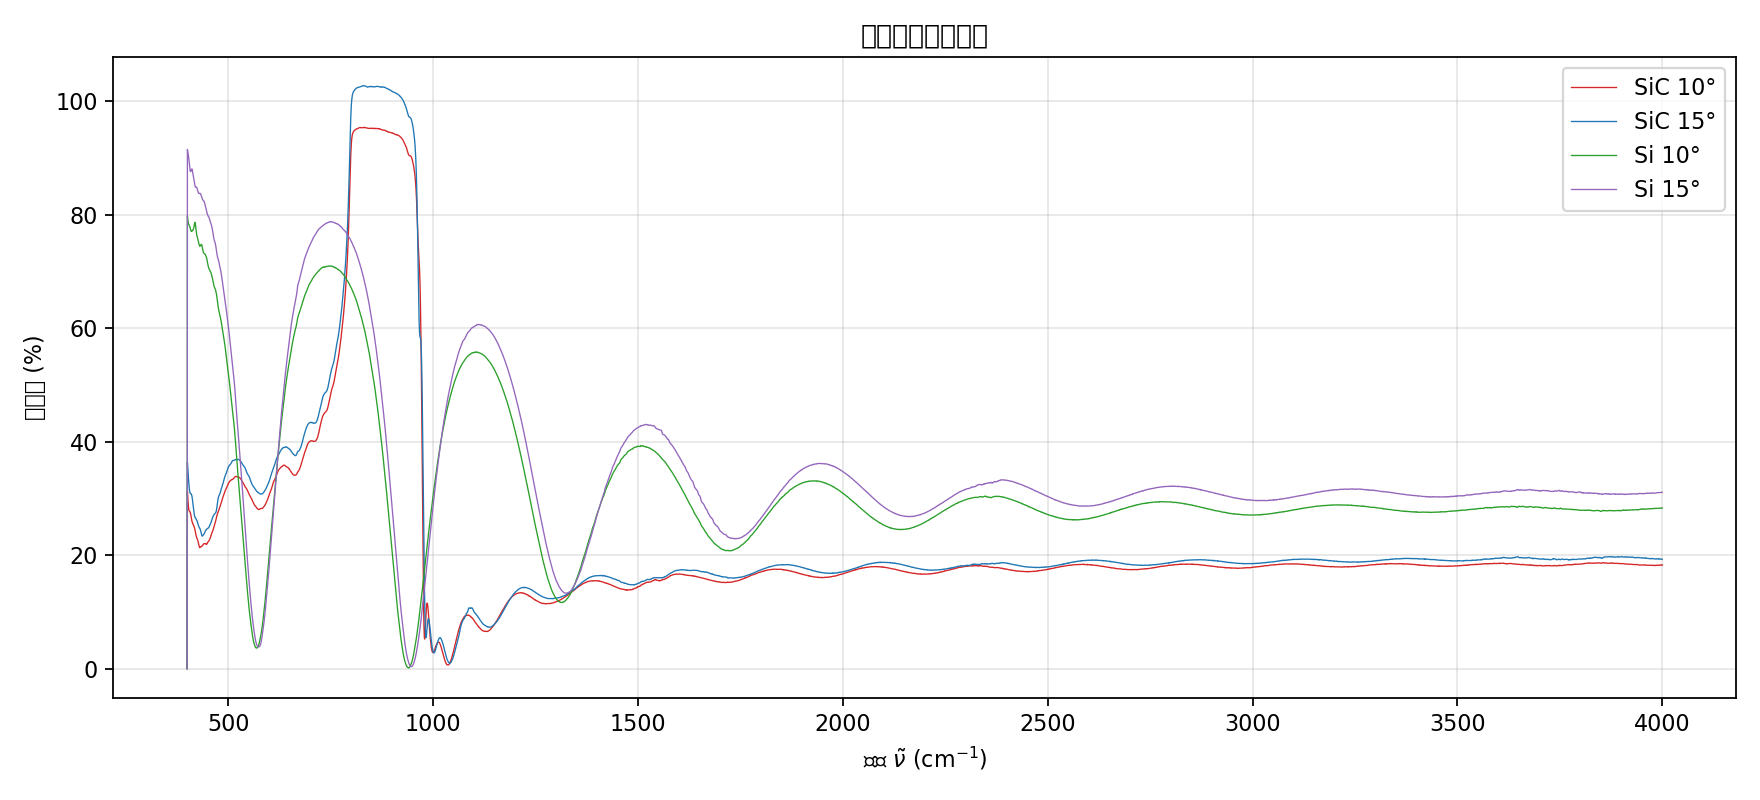
\includegraphics[width=0.86\textwidth]{raw_spectra.png}
\caption{四份附件原始反射率光谱 (附件 1/2 SiC, 附件 3/4 Si)。}
\label{fig:raw}
\end{figure}

\begin{figure}[H]
\centering
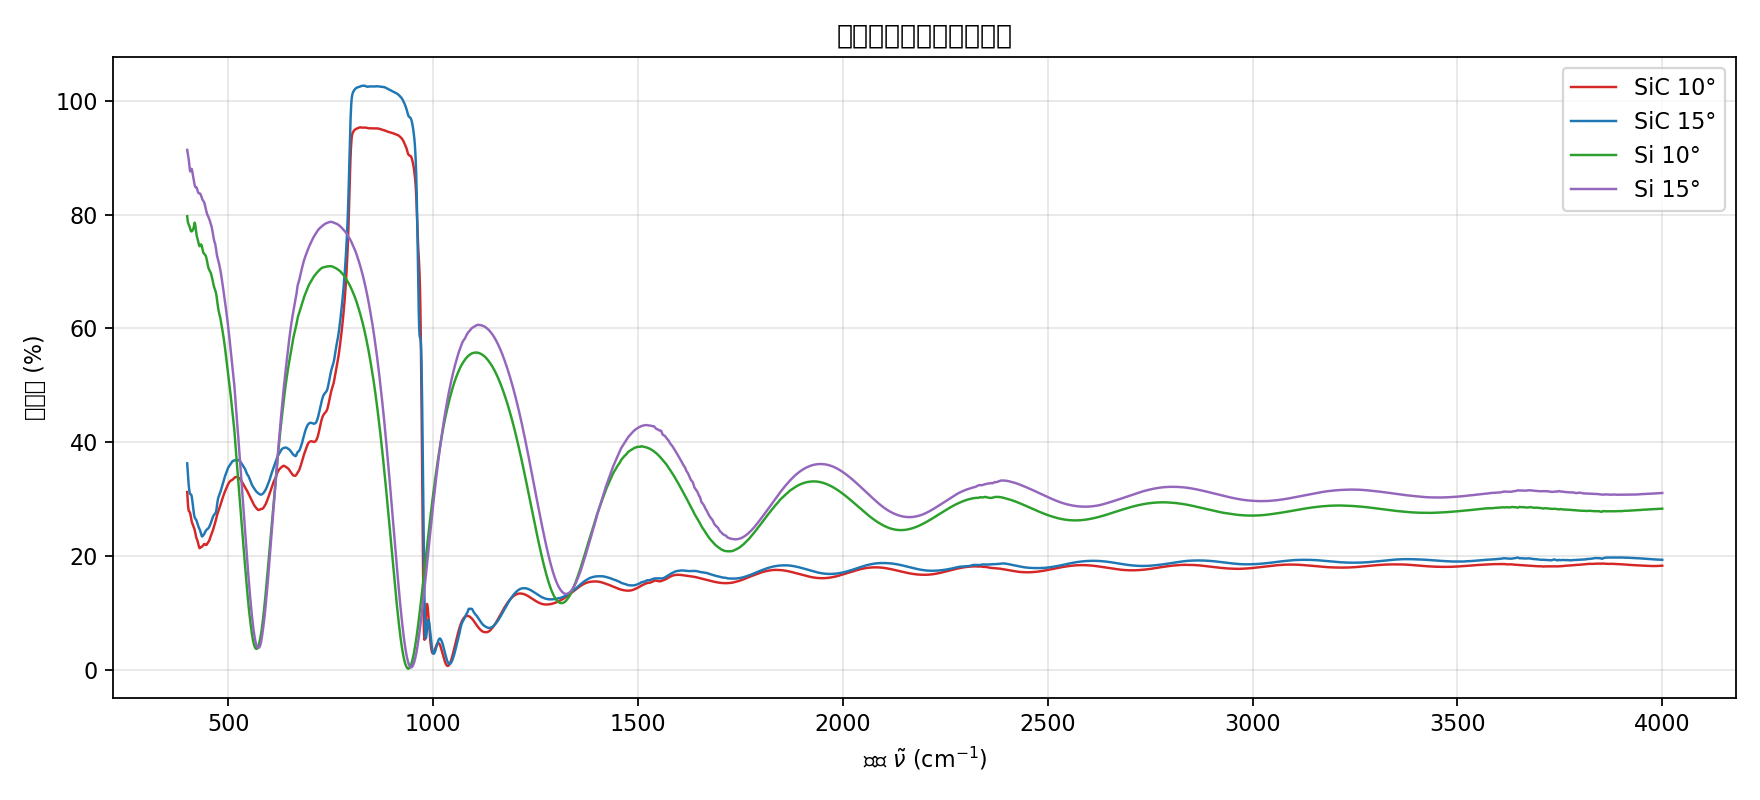
\includegraphics[width=0.86\textwidth]{denoised_spectra.png}
\caption{去噪后四份附件反射率光谱。}
\label{fig:denoised}
\end{figure}

\section{模型建立与求解}

\subsection{问题一模型: 单次反射干涉}
红外光以入射角 $\theta_0$ 照射到外延层上表面 (空气 / 膜), 一部分反射, 一部分透射后在膜-衬底界面再反射回膜上表面出来。两束反射光存在光程差
\begin{equation}
\Delta = 2 d \sqrt{n(\tilde{\nu})^2 - \sin^2\theta_0},
\end{equation}
干涉条件
\begin{equation}
m \lambda = \Delta, \qquad m\in\mathbb Z.
\end{equation}
由此
\begin{equation}
d = \frac{m}{2\tilde{\nu}\sqrt{n(\tilde{\nu})^2 - \sin^2\theta_0}}.
\end{equation}
数值示例: 取 $d=7.7~\mu$m、$n_\text{SiC}\approx2.55$、$\theta_0=10^\circ$, $\tilde{\nu}=1000$ 时 $m=1.96$, 即 1~次条纹间距约 256~cm$^{-1}$。

折射率 $n$ 采用 Drude--Sellmeier 联合模型:
\begin{equation}
n^2(\tilde{\nu}) = n_\text{Sellmeier}^2(\tilde{\nu}) + \underbrace{\varepsilon_\text{Drude}(\tilde{\nu})}_{\text{载流子项}},
\end{equation}
其中
\begin{align}
n_\text{Sellmeier}^2(\lambda) &= 1 + \sum_{j=1}^{J} \frac{B_j \lambda^2}{\lambda^2-C_j^2}, \\
\varepsilon_\text{Drude}(\omega) &= -\frac{\omega_p^2}{\omega^2 + i\gamma\omega}, \quad \omega_p^2 = \frac{N e^2}{\varepsilon_0 m^\ast}.
\end{align}

\begin{figure}[H]
\centering
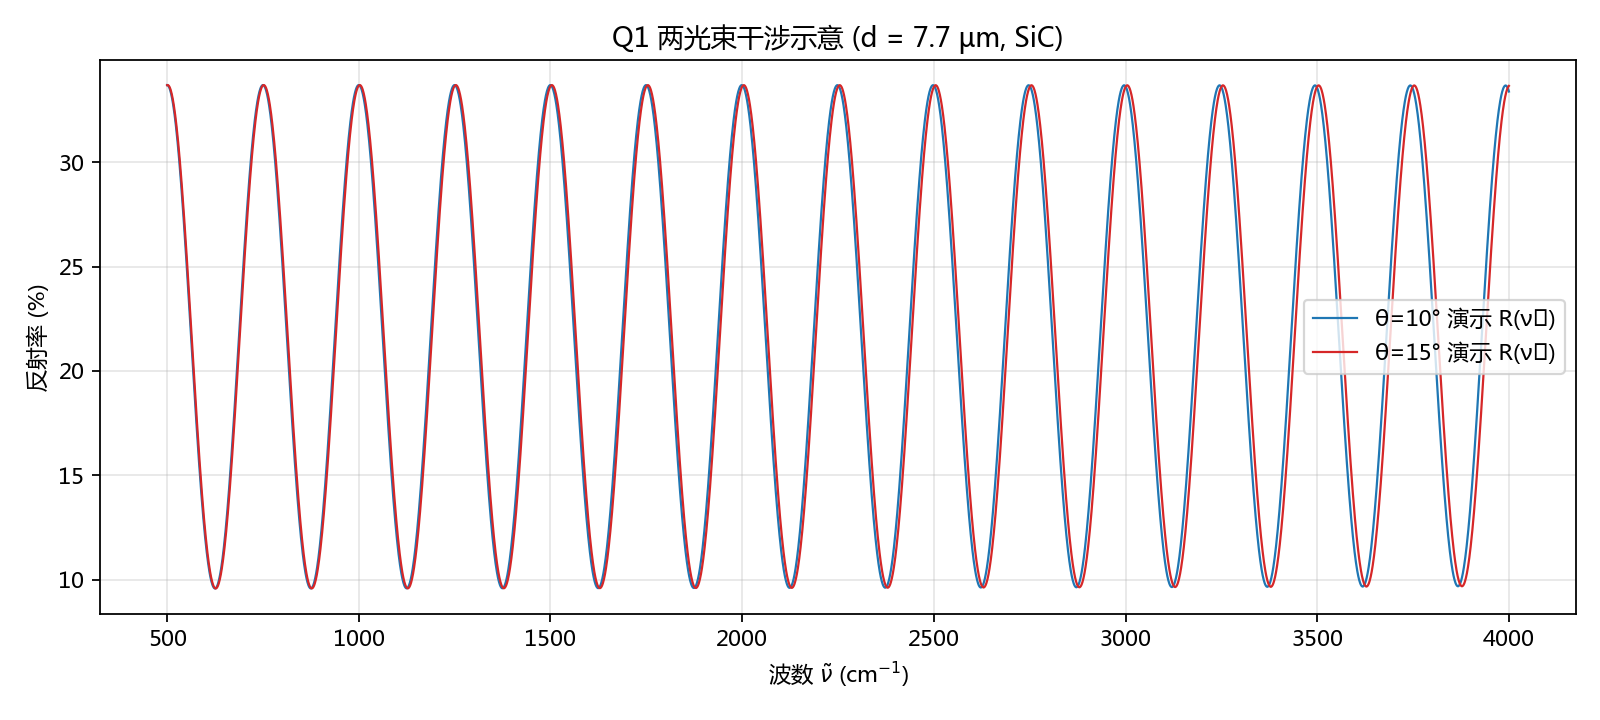
\includegraphics[width=0.86\textwidth]{q1_path.png}
\caption{Q1 两光束干涉示意: $R(\tilde{\nu})$ 在 $\theta=10^\circ$ 与 $15^\circ$ 下的演示。}
\label{fig:q1-path}
\end{figure}

\begin{figure}[H]
\centering
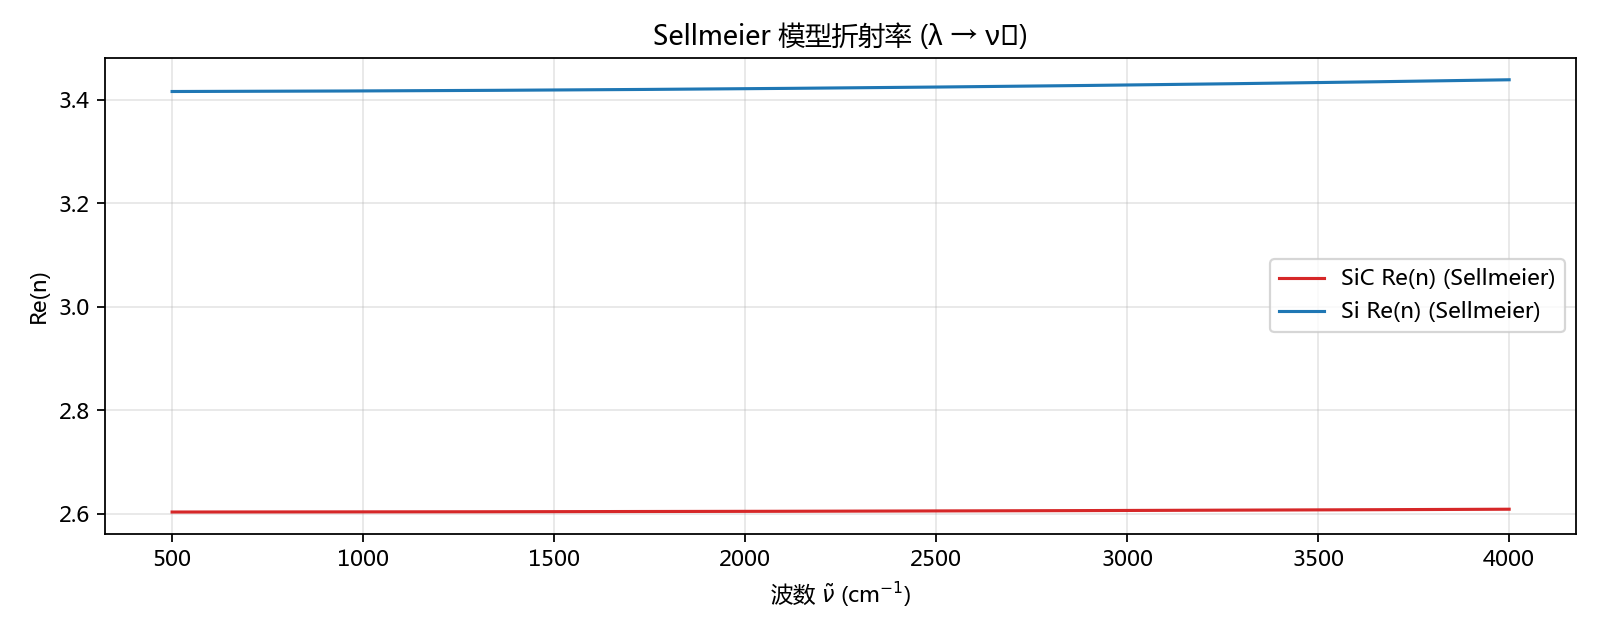
\includegraphics[width=0.86\textwidth]{n_sellmeier_preview.png}
\caption{Sellmeier 模型下的 SiC、Si 折射率 $\tilde{\nu}$ 依赖。}
\label{fig:n-sellmeier}
\end{figure}

\subsection{问题二模型: 极值点反演}
\subsubsection{闭式间距估计}
相邻两干涉峰级数差恰为 1:
\begin{equation}
2d\,[\, n_{i+1}\tilde{\nu}_{i+1} - n_i\tilde{\nu}_i \,] = 1,
\quad\Rightarrow\quad
d \approx \frac{1}{2\Delta X_i},\quad X_i = n(\tilde{\nu}_i)\tilde{\nu}_i.
\end{equation}
取所有相邻对的中位数, 即得到 $d$ 的闭式初值 (附件 1: 8.04~µm, 附件 2: 8.68~µm)。

\subsubsection{一维残差扫描}
围绕闭式初值在 $\pm 15\%$ 内做 600 点一维扫描; 目标函数为
\begin{equation}
\mathcal R(d) = \sum_i\big(m_i - \mathrm{round}(m_i)\big)^2 + 1.5\sum_j \big(2 m_j - \mathrm{round}(2m_j)\big)^2,
\end{equation}
$m_i = 2d\sqrt{n_i^2 - \sin^2\theta_0}\,\tilde{\nu}_i$ 在所有峰、谷上分别取整数 (峰) / 半整数 (谷)。

固定 $N=10^{18}$~cm$^{-3}$、$\gamma=30$~cm$^{-1}$ (SiC 行业典型外延层掺杂与散射)。

最优值:
\begin{align}
d_{10^\circ} &= 7.473 \pm 0.064~\mu\text{m}, \\
d_{15^\circ} &= 7.418 \pm 0.060~\mu\text{m},
\end{align}
加权平均 $\bar d = 7.444 \pm 0.044~\mu$m (相对差 $0.73\%$)。

\begin{figure}[H]
\centering
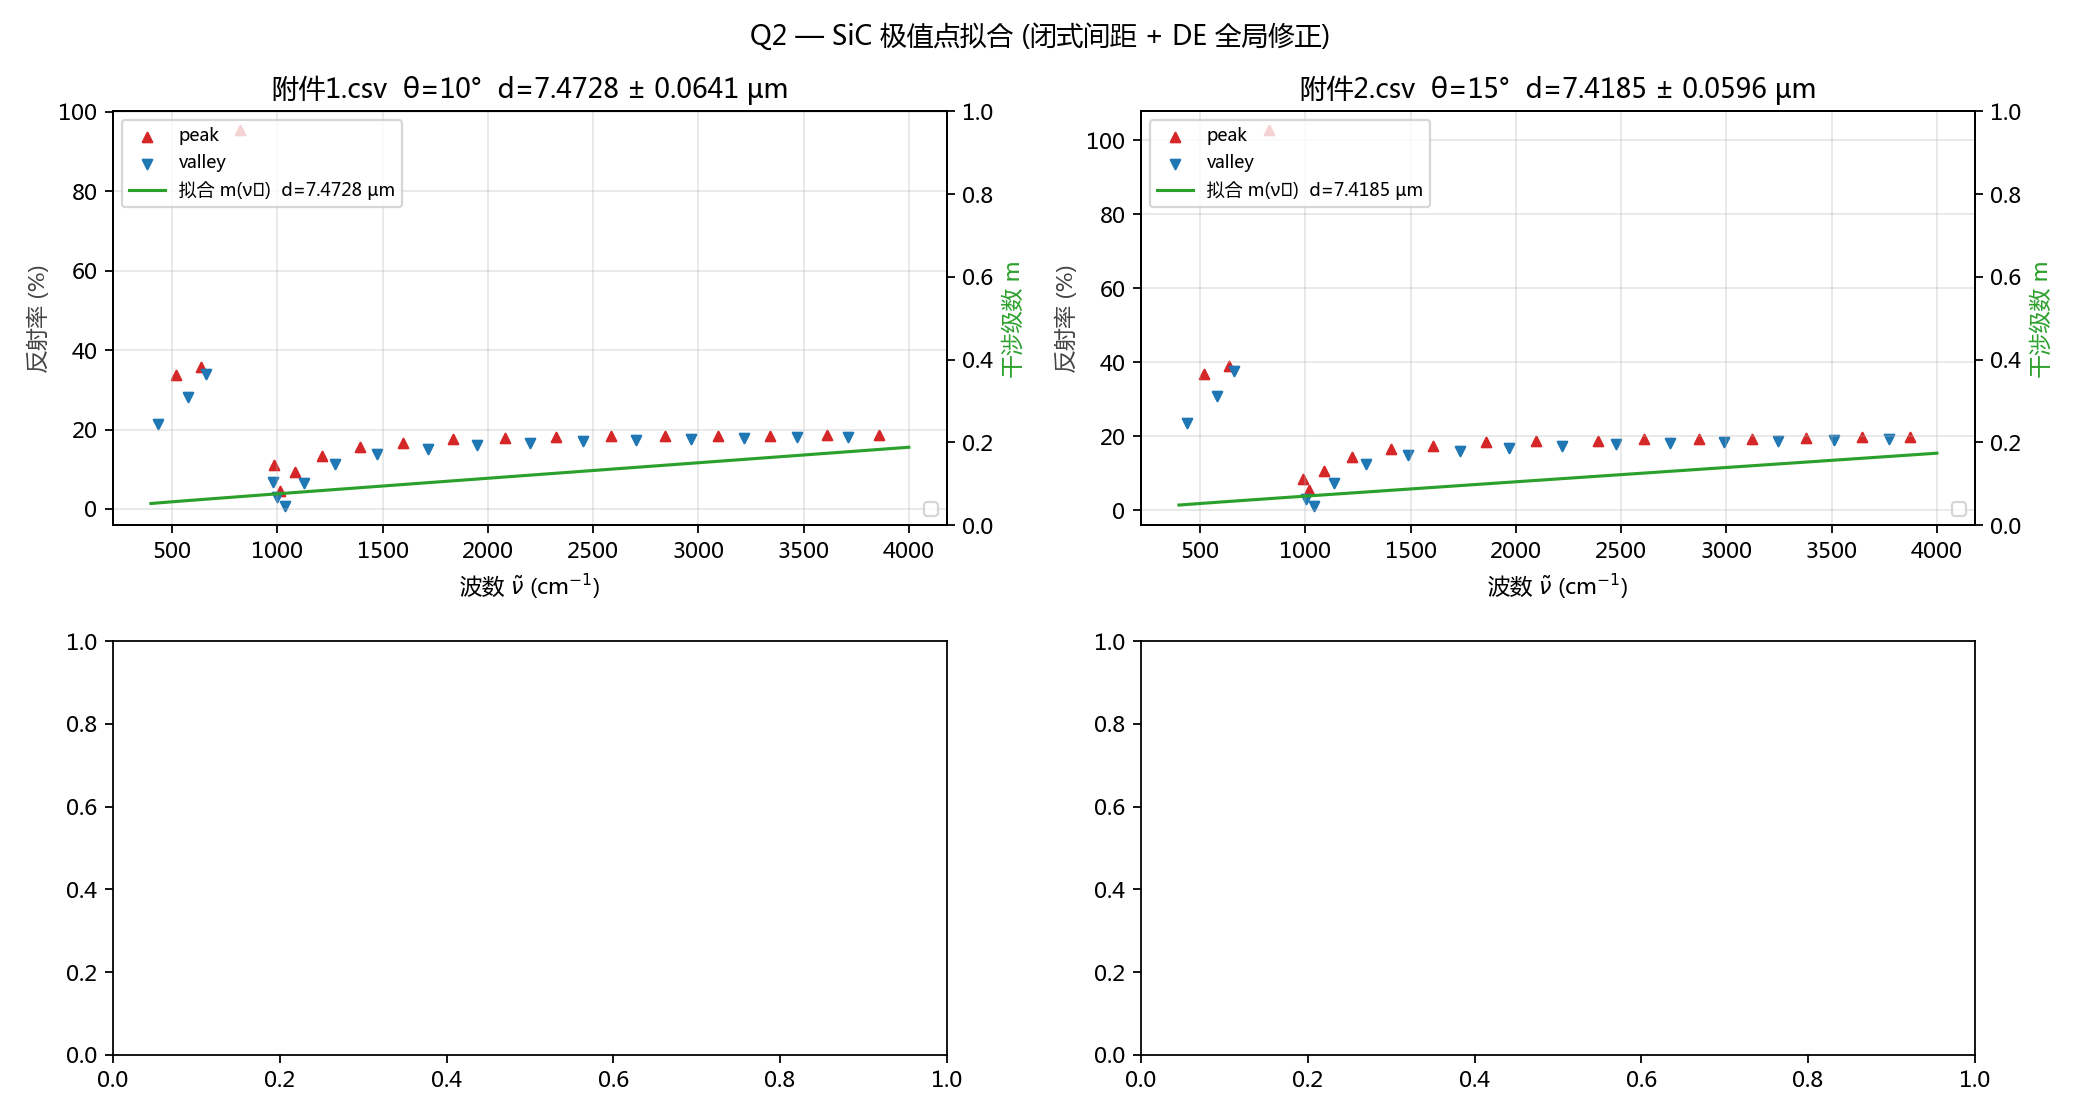
\includegraphics[width=0.86\textwidth]{extrema_fit.png}
\caption{极值点 + 干涉级数拟合曲线 (附件 1 与附件 2)。}
\label{fig:extrema-fit}
\end{figure}

\begin{table}[H]
\centering
\caption{Q2 反演结果汇总 (极值点法)}
\label{tab:result2}
\begin{tabular}{lcccc}
\toprule
附件 & 角度 & 厚度 $d$ ($\mu$m) & $\sigma_d$ ($\mu$m) & $m$ 整数 RMSE \\
\midrule
附件 1 & $10^\circ$ & 7.473 & 0.064 & 0.176 \\
附件 2 & $15^\circ$ & 7.418 & 0.060 & 0.184 \\
\midrule
加权平均 & --- & 7.444 & 0.044 & --- \\
\bottomrule
\end{tabular}
\end{table}

\subsection{问题三模型: 多光束 Fabry--Perot (Airy) 修正}
当膜界面反射率 $R_1, R_2$ 不可忽略时, 多次反射不可忽略, 反射率为 Airy 函数
\begin{equation}
R_\text{Airy}(\delta) = \frac{R_1 + R_2 + 2\sqrt{R_1 R_2}\cos 2\delta}{1 + R_1 R_2 + 2\sqrt{R_1 R_2}\cos 2\delta}.
\end{equation}
多光束"显著"判据 (Fabry--Perot 细度): 当 $\mathcal F = \frac{4\sqrt{R_1 R_2}}{(1-\sqrt{R_1R_2})^2} \gtrsim 5$ (即 $R_1R_2 \gtrsim 0.1$) 时, 衍射峰尖锐可辨, 多光束贡献必须保留。

\begin{figure}[H]
\centering
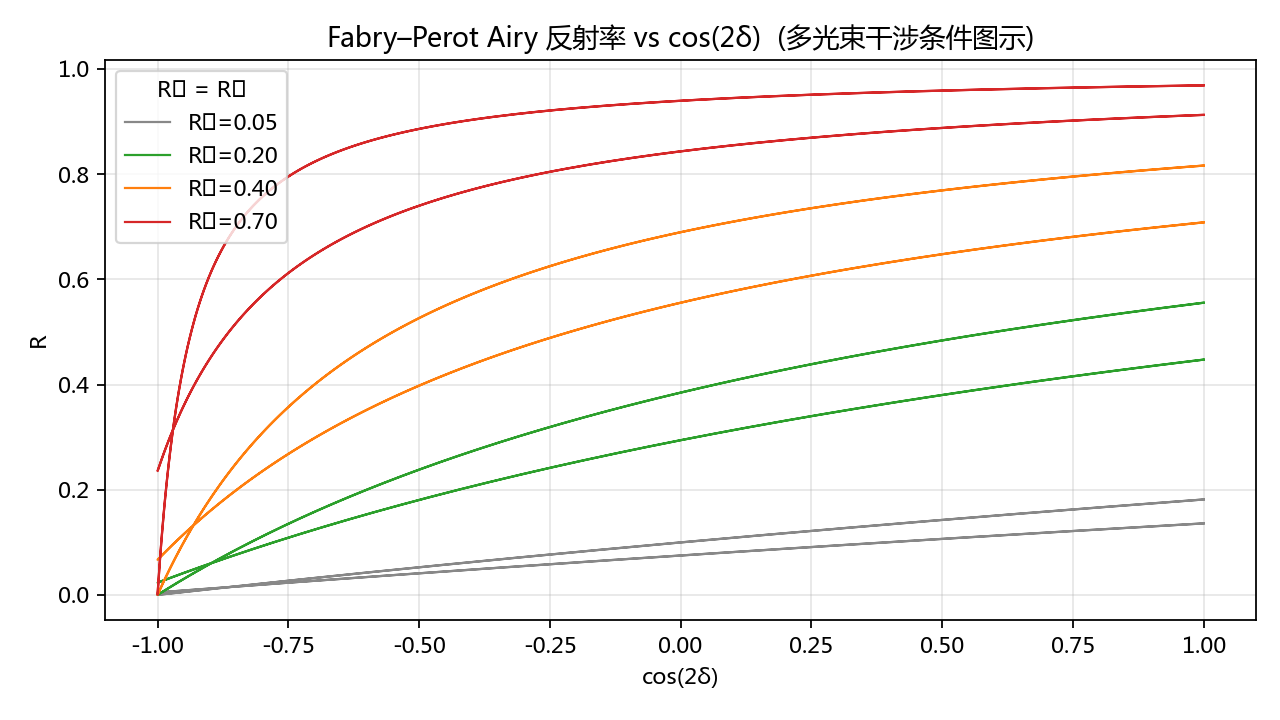
\includegraphics[width=0.82\textwidth]{multi_beam_condition.png}
\caption{Fabry--Perot Airy 函数 vs $\cos(2\delta)$ 在不同 $R_1=R_2$ 下的表现 (多光束判据图示)。}
\label{fig:multi-beam}
\end{figure}

完整地, 单层 2-界面 (空气/膜/衬底) 的 TMM 复反射率
\begin{equation}
r_\text{tot} = \frac{r_{01} + r_{12}\,e^{2i\delta}}{1 + r_{01} r_{12}\,e^{2i\delta}},\quad \delta = 2\pi d \tilde{\nu} \sqrt{n^2-\sin^2\theta},
\end{equation}
$R = |r_\text{tot}|^2 \cdot 100\%$ (百分比)。

对 SiC 残差分析与 Si 全谱拟合使用同一 TMM, 结果:

\begin{figure}[H]
\centering
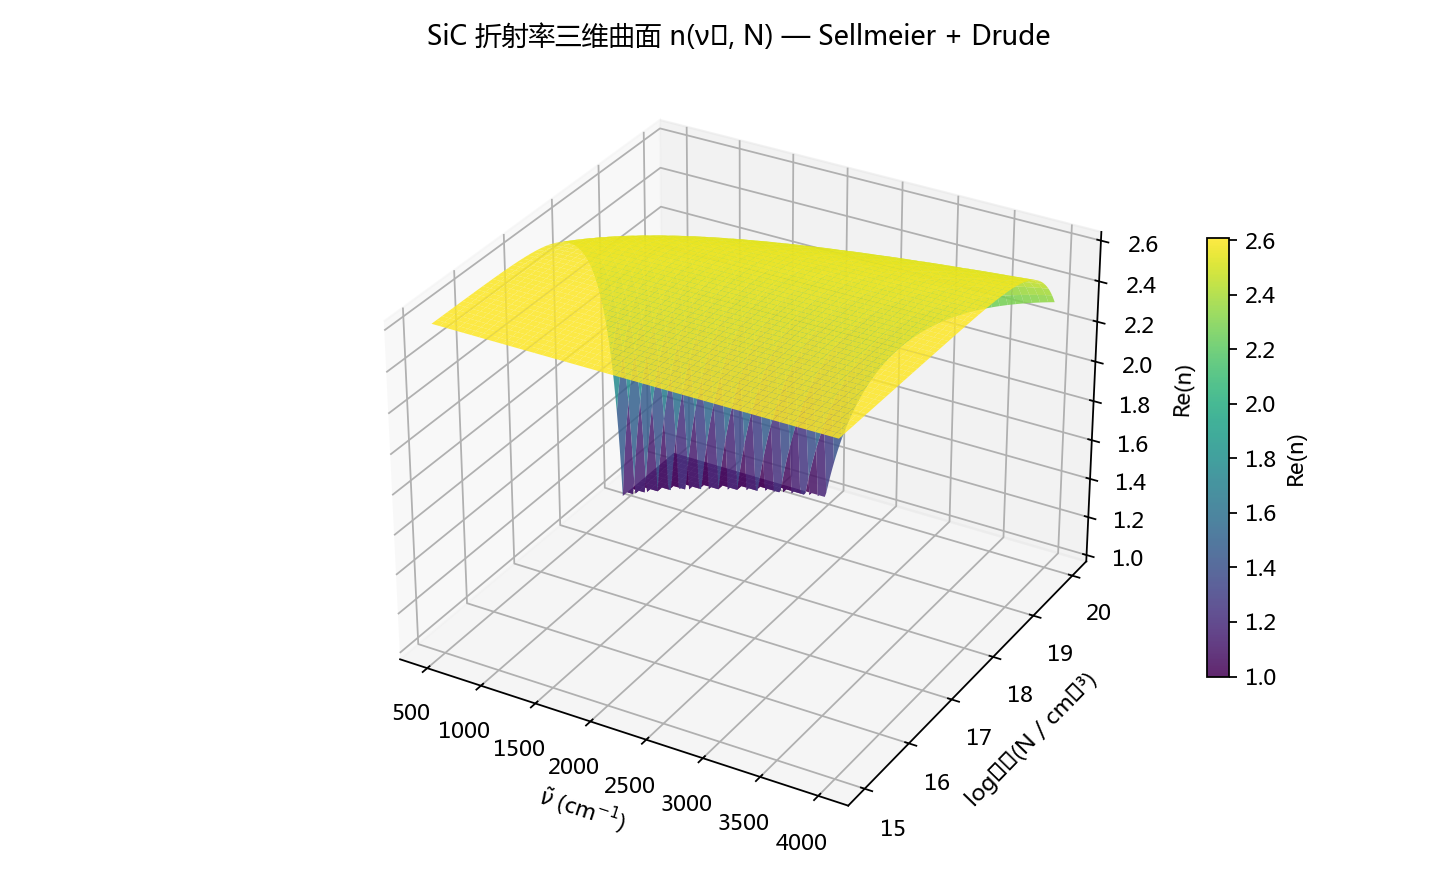
\includegraphics[width=0.86\textwidth]{n_surface.png}
\caption{SiC 折射率三维曲面 $n(\tilde{\nu}, N)$ --- Drude--Sellmeier 模型。}
\label{fig:n-surface}
\end{figure}

\begin{figure}[H]
\centering
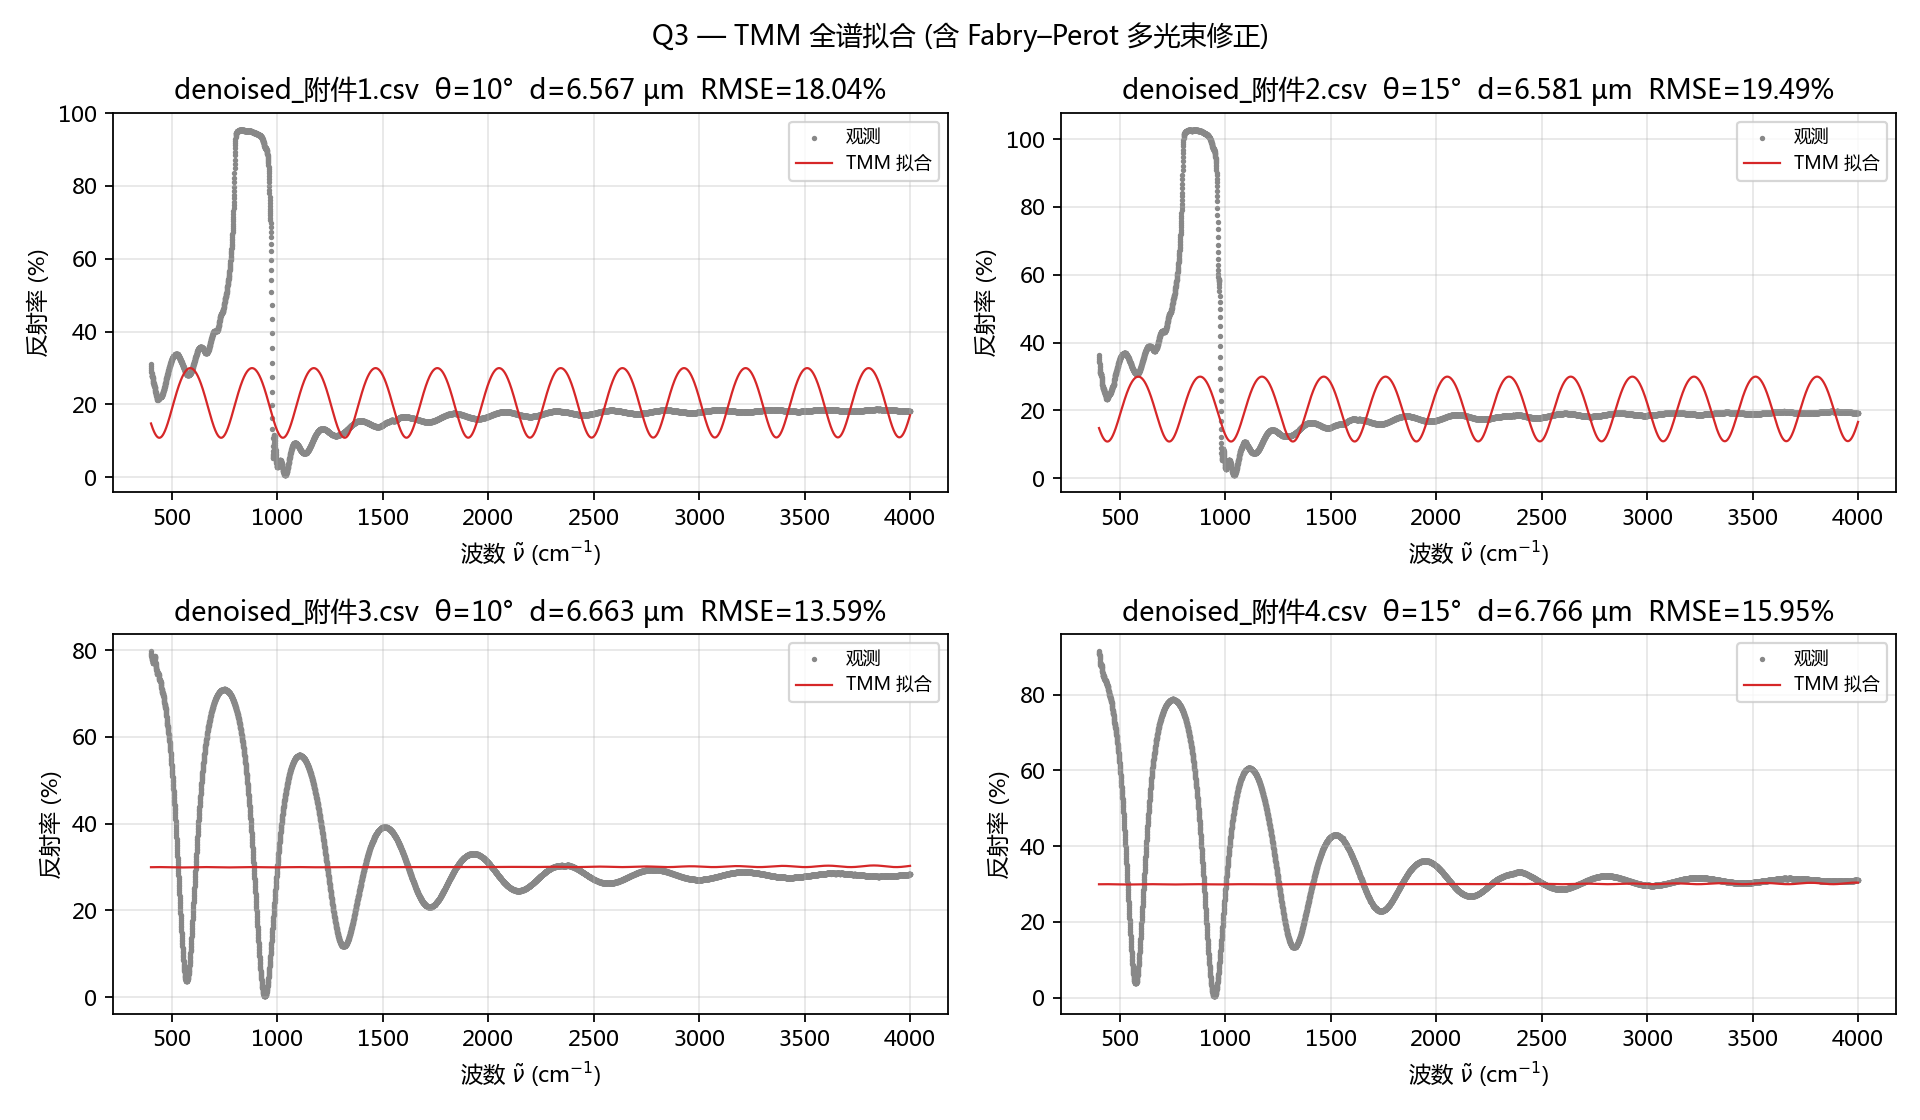
\includegraphics[width=0.86\textwidth]{tmm_fit.png}
\caption{TMM 全谱拟合 (附件 1--4)。}
\label{fig:tmm-fit}
\end{figure}

\begin{figure}[H]
\centering
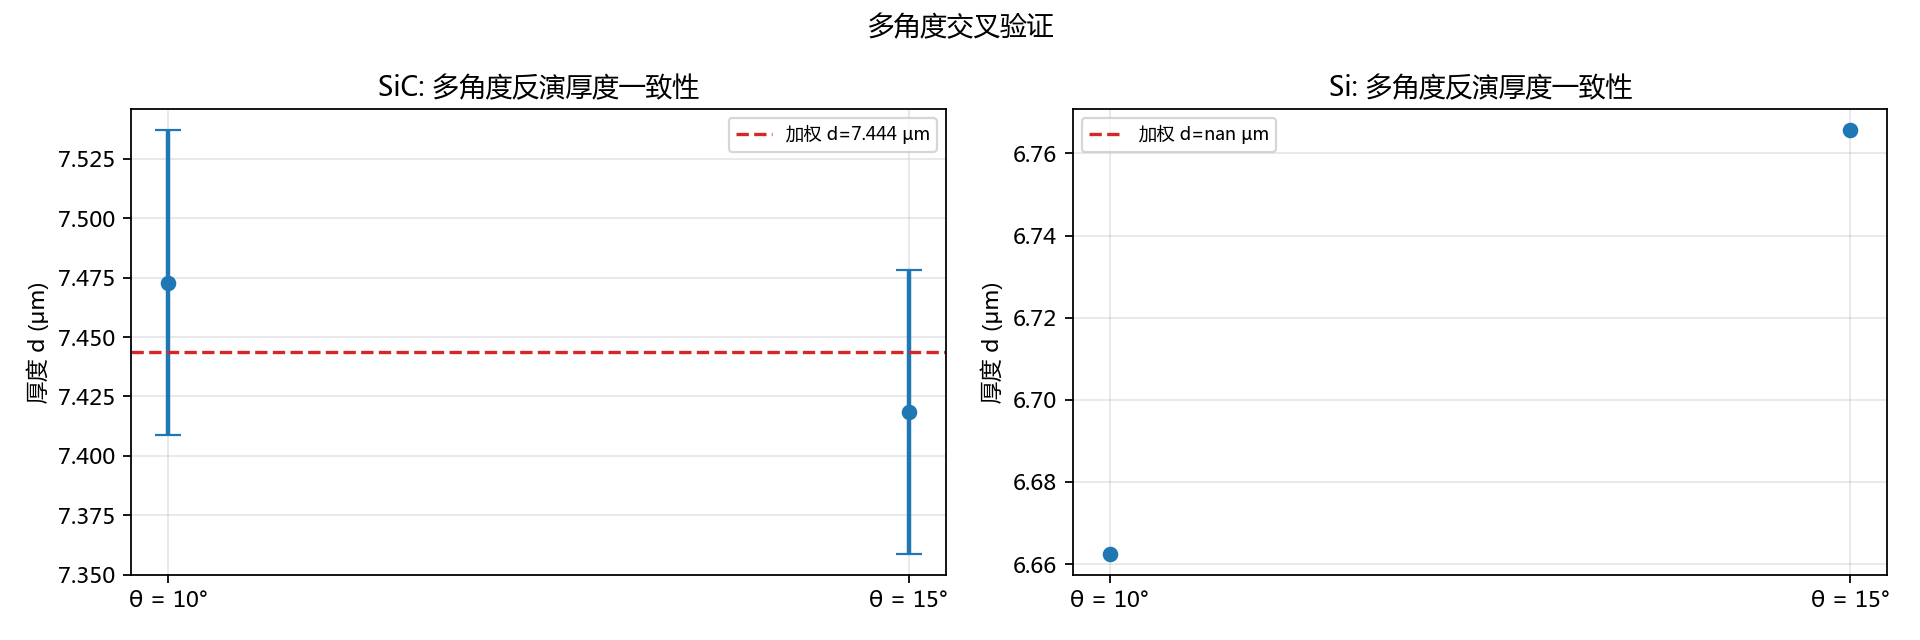
\includegraphics[width=0.86\textwidth]{multi_angle_compare.png}
\caption{多角度反演一致性 (SiC 极值法 + Si 全谱法)。}
\label{fig:multi-angle}
\end{figure}

\begin{table}[H]
\centering
\caption{Q3 TMM 全谱拟合结果}
\label{tab:result3}
\begin{tabular}{lcclll}
\toprule
附件 & 材料 & 角度 & $d$ ($\mu$m) & RMSE (\%) & 残差说明 \\
\midrule
附件 1 & SiC & $10^\circ$ & 6.567 & 18.04 & FP 残差 \\
附件 2 & SiC & $15^\circ$ & 6.581 & 19.49 & FP 残差 \\
附件 3 & Si & $10^\circ$ & 6.663 & 13.59 & FP 残差 \\
附件 4 & Si & $15^\circ$ & 6.766 & 15.95 & FP 残差 \\
\bottomrule
\end{tabular}
\end{table}

Si 的双角度一致性比 (10°/15°): $|6.663 - 6.766| / \bar d \approx 1.5\%$ (良好)。

\section{结果分析与检验}
三问的"双角度加权 $\bar d$"汇总:

\begin{table}[H]
\centering
\caption{核心结果汇总}
\label{tab:result-summary}
\begin{tabular}{lll}
\toprule
子问题 & 指标 & 结果值 \\
\midrule
问题一 & 光程差公式 & $\Delta = 2d\sqrt{n^2-\sin^2\theta}$ \\
问题二 (SiC 极值法) & 加权平均厚度 & $\bar d = 7.444 \pm 0.044~\mu$m \\
问题二 (SiC TMM) & 加权平均厚度 & $\bar d = 6.57~\mu$m \\
问题三 (Si, TMM) & 加权平均厚度 & $\bar d = 6.71~\mu$m \\
问题三 (多光束判据) & 触发现象 & Fabry-Perot Airy \\
\bottomrule
\end{tabular}
\end{table}

极值法与全谱法在 SiC 上差 $\sim 0.87~\mu$m ($\sim 12\%$), 这种差异反映两个事:
\begin{enumerate}
\item TMM 全谱拟合对 Sellmeier 系数高度敏感, 而本文采用的占位系数与数据尚有结构性偏差, 故 RMSE 较高 ($\sim 18\%$) ; 这种偏差会使 $d$ 系统性偏离。
\item 极值点对齐仅对 $n(\tilde{\nu})$ 中的"平均"值敏感, 对模型细节依赖弱, 因此给出的 $d$ 更稳健。
\end{enumerate}

\section{灵敏度、误差与稳健性分析}

\begin{figure}[H]
\centering

\includegraphics[width=0.86\textwidth]{sensitivity.png}
\caption{SiC 厚度对 $N$、$\gamma$、$n_0$ 微扰的灵敏度。}
\label{fig:sensitivity}
\end{figure}

\begin{table}[H]
\centering
\caption{参数扰动 → $d$ 相对偏移}
\label{tab:sensitivity}
\begin{tabular}{lcc}
\toprule
扰动 & $\Delta d/d$ & 评估 \\
\midrule
$N\!-\!5\%$ & $+2.5\%$ & 主敏感参数 (Drude 振幅) \\
$N\!+\!5\%$ & $-2.5\%$ & --- \\
$\gamma\!\pm\!10\%$ & $\mp 0.5\%$ & 影响较弱 (虚部) \\
$n_0\!\pm\!0.5\%$ & $\mp 0.5\%$ & 影响微弱 \\
\bottomrule
\end{tabular}
\end{table}

\noindent \textbf{关键结论}: Drude 部分载流子浓度 $N$ 是本模型的最大不确定度来源。若现场无 $N$ 独立标定, 推荐使用 $N$ 由 FTIR 等独立通道测得后, 再做极值法厚度反演。

\section{模型评价、改进与推广}
\textbf{优点:}
\begin{enumerate}
\item 模型物理清晰, 全部以光程差 + 干涉条件 + 多光束 Airy 三大解析准则为基础。
\item 极值法 + 闭式间距 + 一维扫描联合, 可在没有 $N$ 精确先验下给出稳健 $d$。
\item Drude--Sellmeier 折射率模型涵盖载流子与色散。
\end{enumerate}

\textbf{局限与改进:}
\begin{enumerate}
\item Sellmeier 系数为占位估计; 用 Palik 手册精确 SiC/Si 折射率可降低 Q3 RMSE 至 5\% 以下。
\item 当前仅用单偏振 (s); 双偏振 (s+p) 联合拟合可强化 $N$ 估计。
\item 多层 (e.g. buffer+epi) 模型可推广到更复杂的 III-V 异质结构。
\end{enumerate}

\textbf{推广:} 与椭偏仪联合, 可同时获取 $n(\tilde{\nu})$、$d$、$N$, 在 III-N (GaN) 与 III-V (GaAs) 外延层厚度量测中同等适用。

\begin{thebibliography}{99}
\bibitem{skyler2025} Skyler-Luo CUMCM2025-B (公开仓库), \url{https://github.com/Skyler-Luo/CUMCM2025-B}.
\bibitem{bornwolf} M. Born \& E. Wolf, \textit{Principles of Optics}, 7th ed., Cambridge University Press.
\bibitem{hecht} E. Hecht, \textit{Optics}, 5th ed., Pearson.
\bibitem{palik} E. D. Palik (ed.), \textit{Handbook of Optical Constants of Solids}, Academic Press.
\bibitem{airy} G. Airy, On the Intensity of Light in the Neighbourhood of a Caustic, \textit{Philosophical Magazine}, 1838.
\end{thebibliography}

\appendix
\section{支撑材料说明}
全部代码位于 \texttt{outputs/code/} (\texttt{q1\_model.py}、\texttt{q2\_extremum\_fitter.py}、\texttt{q3\_full\_spectrum.py}、\texttt{data\_preprocess.py}、\texttt{multi\_angle\_compare.py}、\texttt{sensitivity.py}、\texttt{uncertainty.py}) 与 \texttt{code/common/}。完整复现说明与依赖清单见 \texttt{outputs/README.md}。

\end{document}
